%%%%%%%%%%%%%%%%
%% Preambule  %%
%%%%%%%%%%%%%%%%

\documentclass[11pt]{article}

\usepackage{amsmath,amsfonts,amssymb}
\usepackage{upgreek}
\usepackage{enumerate}
\usepackage{enumitem}
\usepackage{multicol}
\usepackage{scrextend}

\usepackage[all]{xy}
\usepackage{tikz-qtree}
\usepackage[margin=2.5cm]{geometry}

\usepackage{fancyhdr}
\usepackage{lastpage}
\usepackage{subcaption}

\setlength{\parindent}{0pt}

\pagestyle{fancy}

\lhead{\opdrachtNaam\ \opdrachtNummer}
\rhead{\naam(\studentNummer)}
\rfoot{Page\ \thepage\ of\ \pageref{LastPage}}
\lfoot{\datum}
\cfoot{}

\renewcommand\headrulewidth{0.4pt}
\renewcommand\footrulewidth{0.4pt}

\newcommand{\E}{\exists}
\newcommand{\A}{\forall}


\newcommand{\ccen}[2]{\llap{$#1$}${}\mathrel{\circ}{}$\rlap{$#2$}}


%%%%%%%%%%%%%%
%% Gegevens %%
%%%%%%%%%%%%%%

% Vul hier je gegevens in.

\newcommand{\naam}          {Stefan Schenk}
\newcommand{\studentNummer} {11881798}
\newcommand{\opdrachtNaam}  {Assignment}
\newcommand{\opdrachtNummer}{1}
\newcommand{\datum}         {November 2017}


%%%%%%%%%%%%%%%%
%% Antwoorden %%
%%%%%%%%%%%%%%%%

\begin{document}


%%%%%%%%%%%%%%%%
%% Question 1 %%
%%%%%%%%%%%%%%%%

\section*{Question 1}

\begin{enumerate}[label=(\alph*)]

  \item Produce clear images for the surface plots for both Model CT and Model
  D, and provide screenshots for the input membership functions as well as the
  output membership functions. State your answers clearly for each model,
  separately.

  \begin{figure}[ht!]
  \centering
  \begin{subfigure}{.5\textwidth}
    \centering
    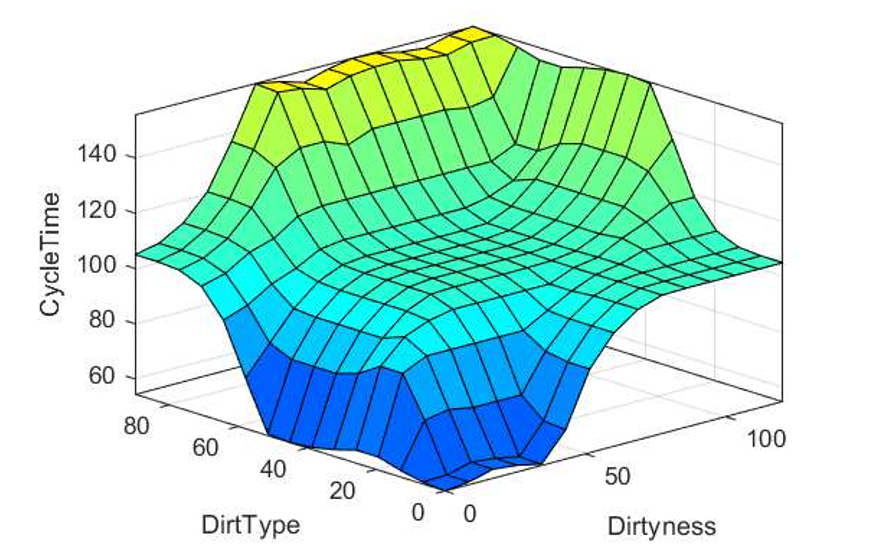
\includegraphics[width=.9\linewidth]{res/image1}
    \caption{ModelCT}
    \label{fig:sub1}
  \end{subfigure}%
  \begin{subfigure}{.5\textwidth}
    \centering
    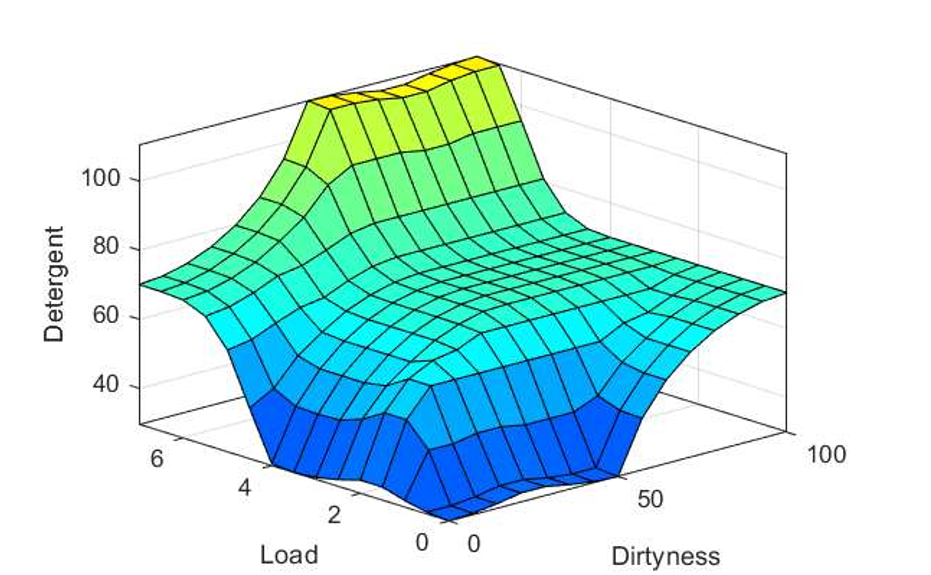
\includegraphics[width=.9\linewidth]{res/image2}
    \caption{ModelD}
    \label{fig:sub2}
  \end{subfigure}
  \end{figure}

  \begin{figure}[ht!]
  \centering
  \begin{subfigure}{.5\textwidth}
    \centering
    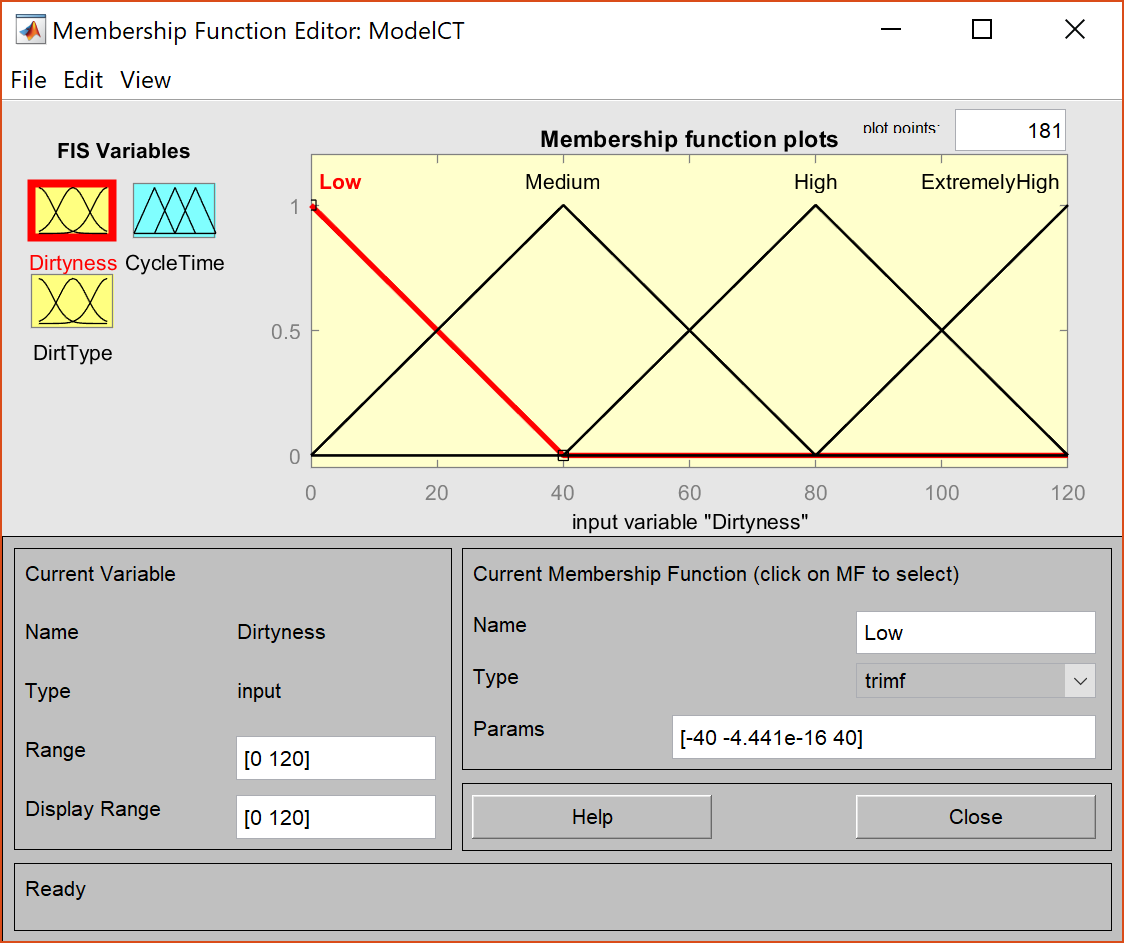
\includegraphics[width=.9\linewidth]{res/image1_dirtyness}
    \caption{ModelCT - Dirtyness Input}
    \label{fig:sub1}
  \end{subfigure}%
  \begin{subfigure}{.5\textwidth}
    \centering
    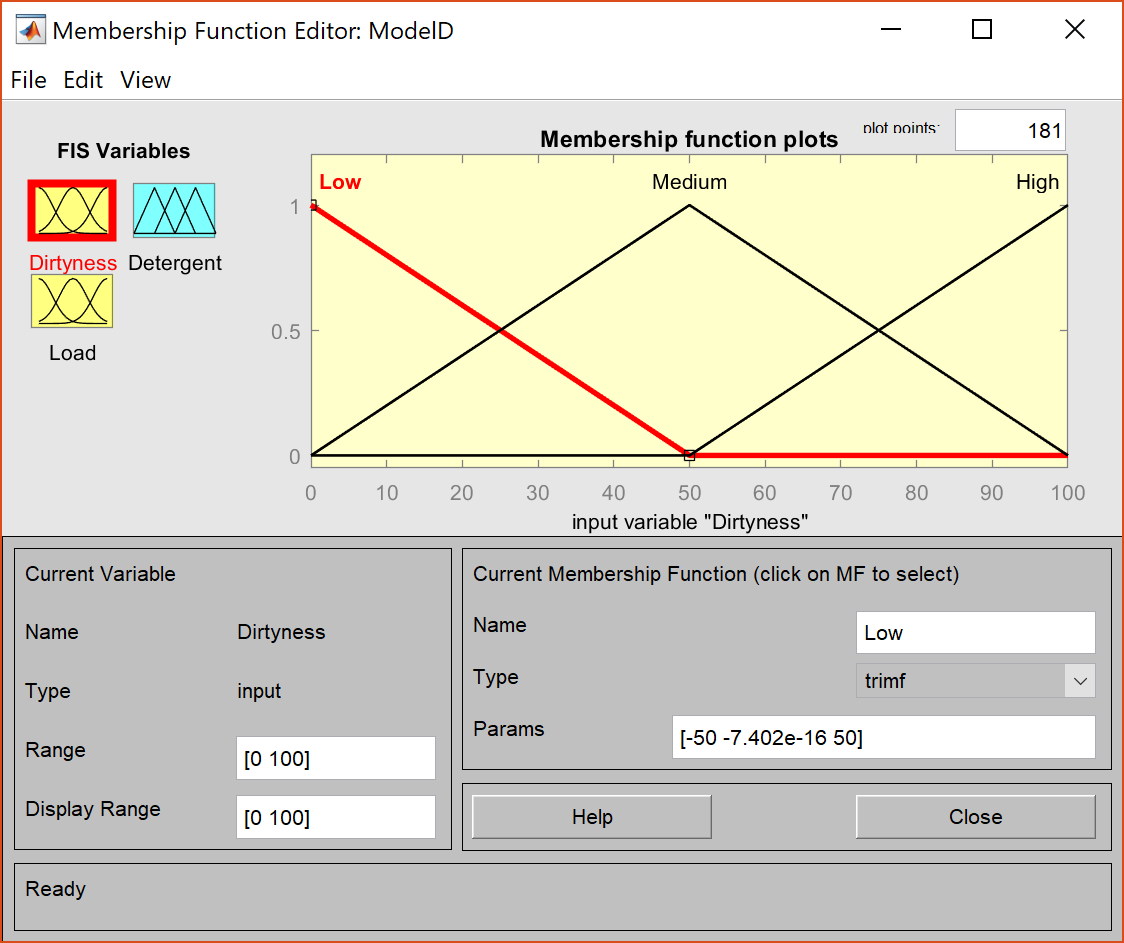
\includegraphics[width=.9\linewidth]{res/image2_dirtyness}
    \caption{ModelD - Dirtyness Input}
    \label{fig:sub2}
  \end{subfigure}
  \end{figure}

  \begin{figure}[ht!]
  \centering
  \begin{subfigure}{.5\textwidth}
    \centering
    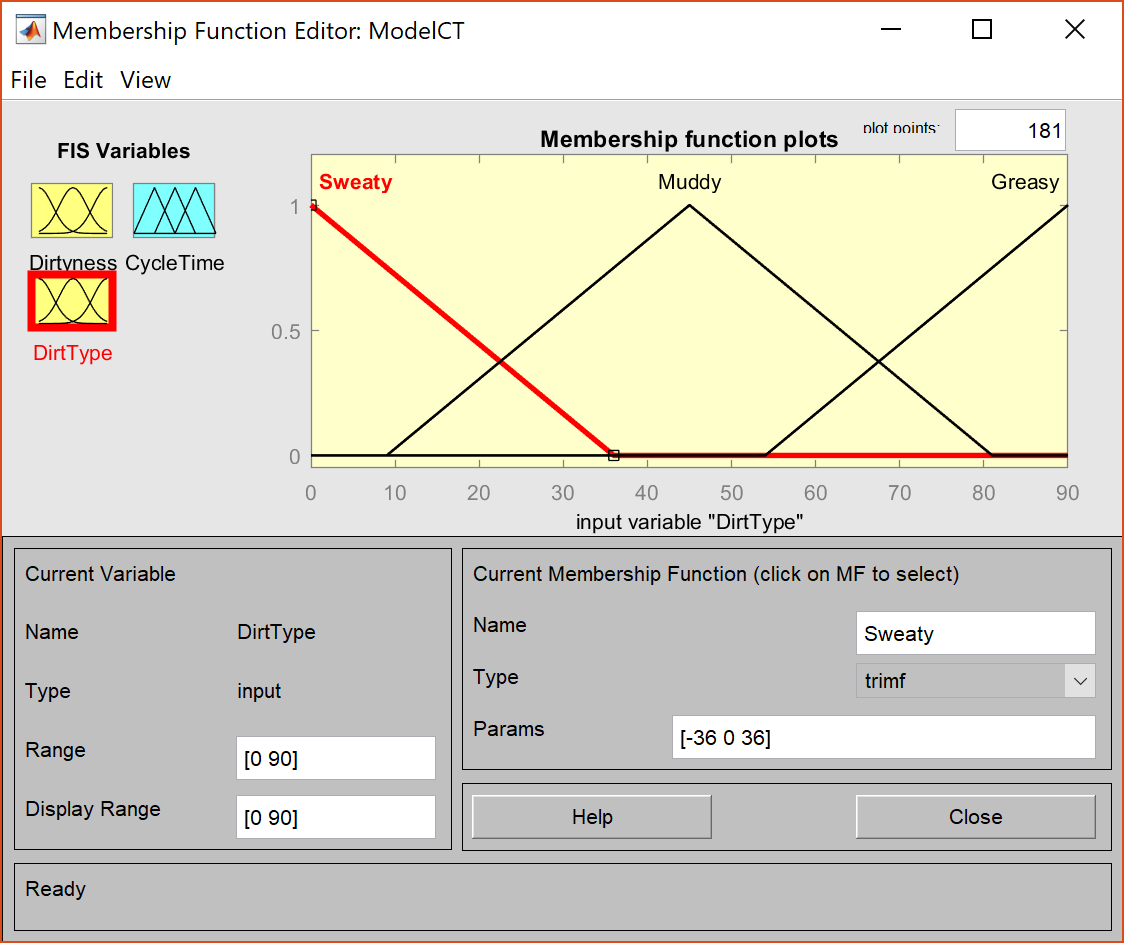
\includegraphics[width=.9\linewidth]{res/image1_dirttype}
    \caption{ModelCT - DirtType Input}
    \label{fig:sub1}
  \end{subfigure}%
  \begin{subfigure}{.5\textwidth}
    \centering
    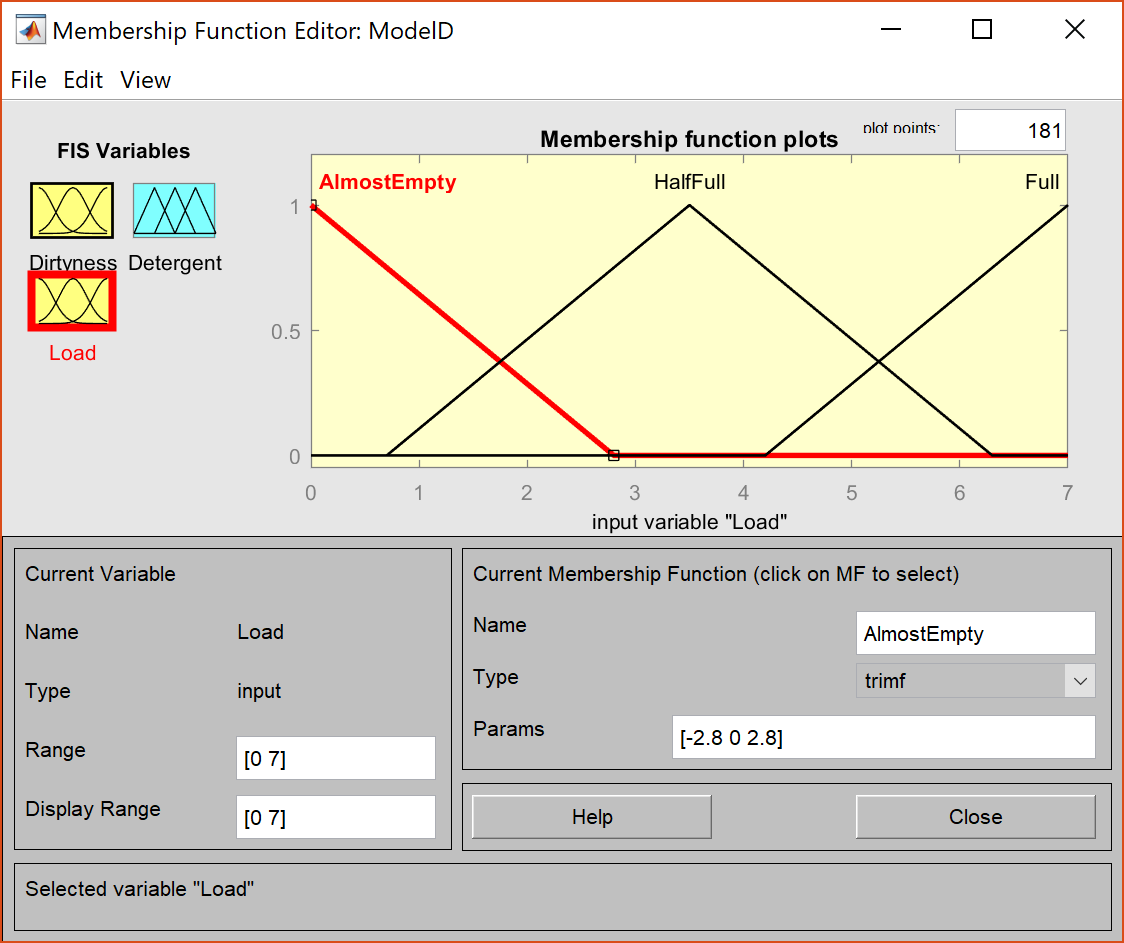
\includegraphics[width=.9\linewidth]{res/image2_load}
    \caption{ModelD - Load Input}
    \label{fig:sub2}
  \end{subfigure}
  \end{figure}

  \begin{figure}[ht!]
  \centering
  \begin{subfigure}{.5\textwidth}
    \centering
    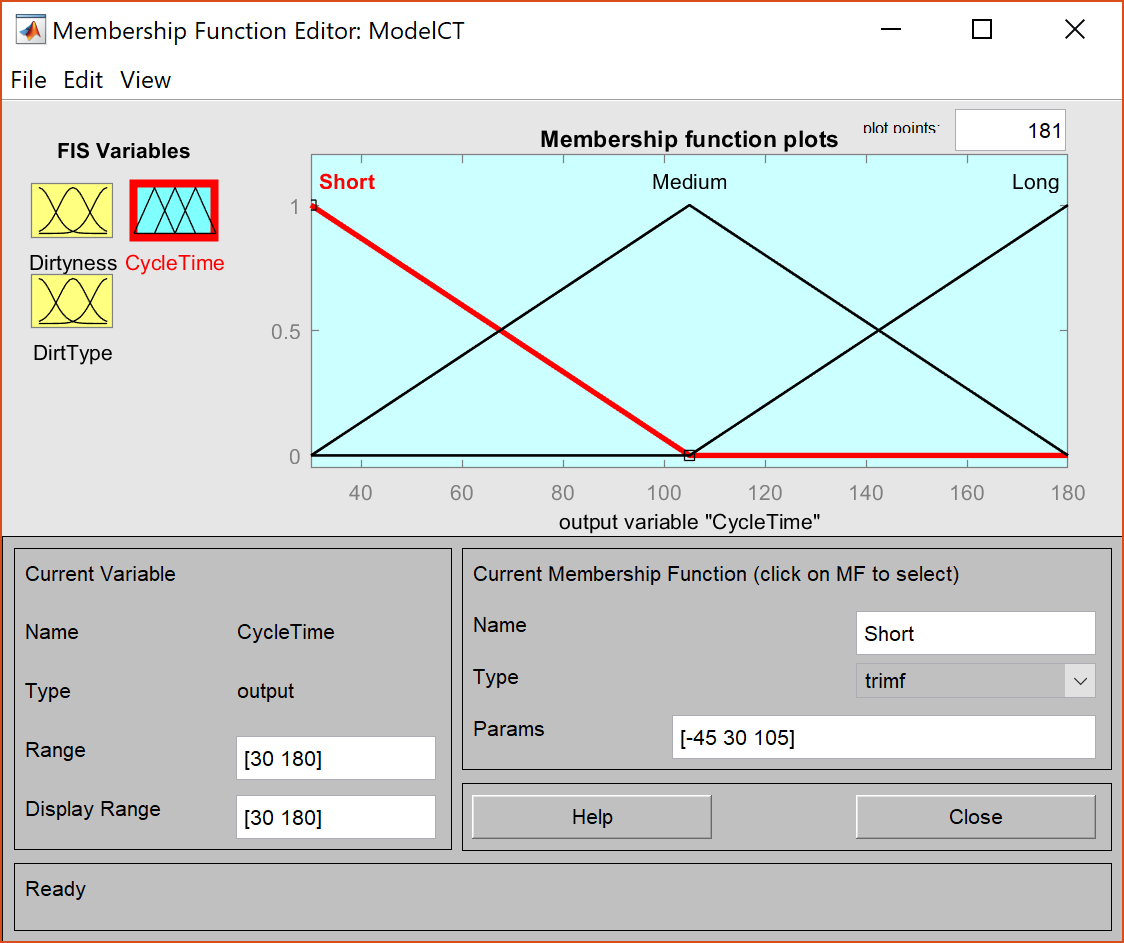
\includegraphics[width=.9\linewidth]{res/image1_cycletime}
    \caption{ModelCT - CycleTime Output}
    \label{fig:sub1}
  \end{subfigure}%
  \begin{subfigure}{.5\textwidth}
    \centering
    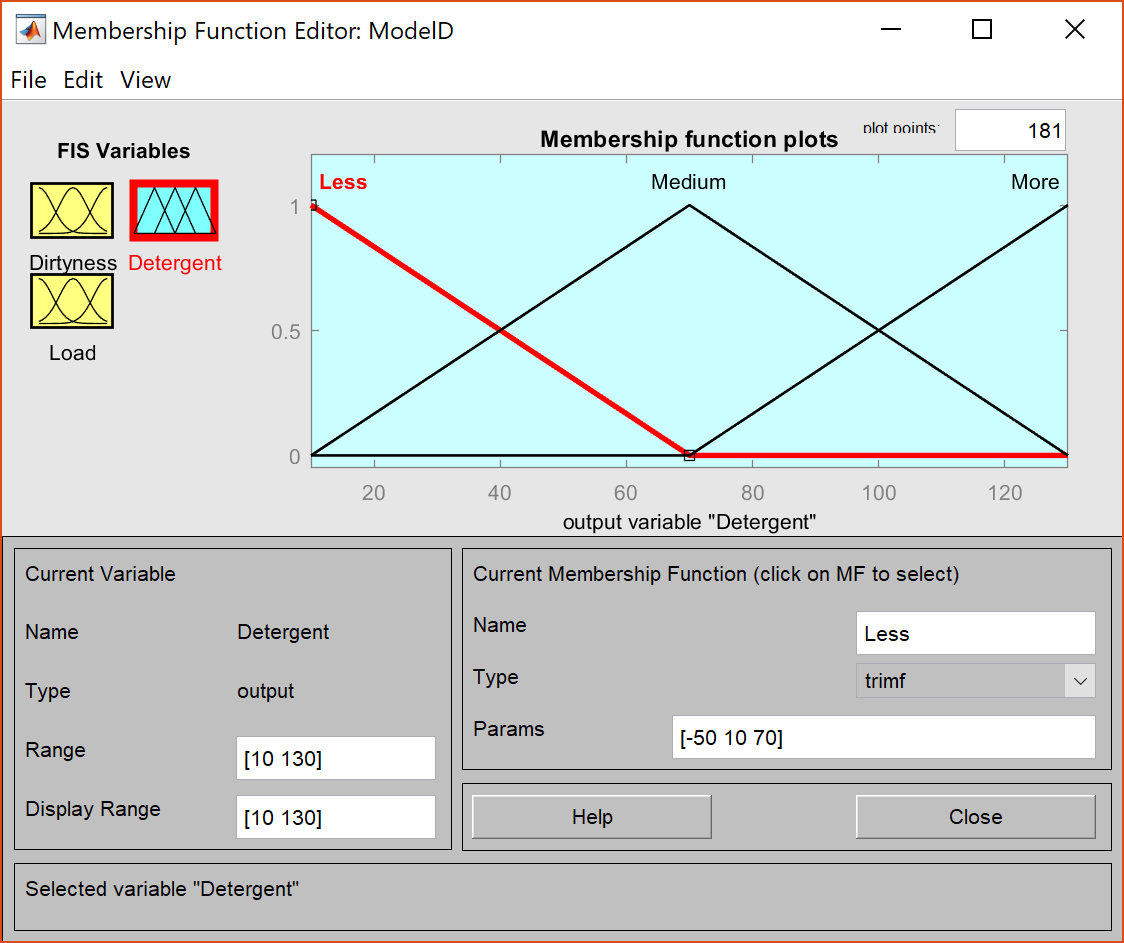
\includegraphics[width=.9\linewidth]{res/image2_detergent}
    \caption{ModelD - Detergent Output}
    \label{fig:sub2}
  \end{subfigure}
  \end{figure}

  \pagebreak

  \item Modify the rule bases for both Model CT and Model D by reducing as much
  rules as possible, without changing the behaviour of the system too much. How
  would you explain the behaviour change while logically maintaining the rule
  base? If this is possible, give an example of your reasoning. Report the new
  rule bases, separately, and justify your decisions by briefly describing your
  motivation.

  Using the not box, it is possible to avoid make rules seperately for each
  non-changing variable, reducing the number of rules from 9 to 6 for ModelD, and from 12 to 10 for ModelCT.

  \subsection*{ModelD}

  Before:
  \begin{enumerate}[label=(\arabic*)]
  \item If (Dirtyness is Low) and (Load is AlmostEmpty) then (Detergent is Less) (1)
  \item If (Dirtyness is Medium) and (Load is AlmostEmpty) then (Detergent is Less) (1)
  \item If (Dirtyness is High) and (Load is AlmostEmpty) then (Detergent is Medium) (1)
  \item If (Dirtyness is Low) and (Load is HalfFull) then (Detergent is Less) (1)
  \item If (Dirtyness is Medium) and (Load is HalfFull) then (Detergent is Medium) (1)
  \item If (Dirtyness is High) and (Load is HalfFull) then (Detergent is Medium) (1)
  \item If (Dirtyness is Low) and (Load is Full) then (Detergent is Medium) (1)
  \item If (Dirtyness is Medium) and (Load is Full) then (Detergent is More) (1)
  \item If (Dirtyness is High) and (Load is Full) then (Detergent is More) (1)
  \end{enumerate}

  After:
  \begin{enumerate}[label=(\arabic*)]
  \item If (Dirtyness is not High) and (Load is AlmostEmpty) then (Detergent is Less) (1)
  \item If (Dirtyness is High) and (Load is AlmostEmpty) then (Detergent is Medium) (1)
  \item If (Dirtyness is Low) and (Load is HalfFull) then (Detergent is Less) (1)\item If (Dirtyness is not Low) and (Load is HalfFull) then (Detergent is Medium) (1)
  \item If (Dirtyness is Low) and (Load is Full) then (Detergent is Medium) (1)
  \item If (Dirtyness is not Low) and (Load is Full) then (Detergent is More) (1)
  \end{enumerate}

  \subsection*{ModelCT}

  Before:
  \begin{enumerate}[label=(\arabic*)]
  \item If (Dirtyness is Low) and (DirtType is Sweaty) then (CycleTime is Short) (1)
  \item If (Dirtyness is Medium) and (DirtType is Sweaty) then (CycleTime is Short) (1)
  \item If (Dirtyness is High) and (DirtType is Sweaty) then (CycleTime is Medium) (1)
  \item If (Dirtyness is ExtremelyHigh) and (DirtType is Sweaty) then (CycleTime is Medium) (1)
  \item If (Dirtyness is Low) and (DirtType is Muddy) then (CycleTime is Short) (1)
  \item If (Dirtyness is Medium) and (DirtType is Muddy) then (CycleTime is Medium) (1)
  \item If (Dirtyness is High) and (DirtType is Muddy) then (CycleTime is Medium) (1)
  \item If (Dirtyness is ExtremelyHigh) and (DirtType is Muddy) then (CycleTime is Long) (1)
  \item If (Dirtyness is Low) and (DirtType is Greasy) then (CycleTime is Medium) (1)
  \item If (Dirtyness is Medium) and (DirtType is Greasy) then (CycleTime is Long) (1)
  \item If (Dirtyness is High) and (DirtType is Greasy) then (CycleTime is Long) (1)
  \item If (Dirtyness is ExtremelyHigh) and (DirtType is Greasy) then (CycleTime is Long) (1)
  \end{enumerate}

  After:
  \begin{enumerate}[label=(\arabic*)]
  \item If (Dirtyness is Low) and (DirtType is Sweaty) then (CycleTime is Short) (1)
  \item If (Dirtyness is Medium) and (DirtType is Sweaty) then (CycleTime is Short) (1)
  \item If (Dirtyness is High) and (DirtType is Sweaty) then (CycleTime is Medium) (1)
  \item If (Dirtyness is ExtremelyHigh) and (DirtType is Sweaty) then (CycleTime is Medium) (1)
  \item If (Dirtyness is Low) and (DirtType is Muddy) then (CycleTime is Short) (1)\item If (Dirtyness is Medium) and (DirtType is Muddy) then (CycleTime is Medium) (1)
  \item If (Dirtyness is High) and (DirtType is Muddy) then (CycleTime is Medium) (1)
  \item If (Dirtyness is ExtremelyHigh) and (DirtType is Muddy) then (CycleTime is Long) (1)
  \item If (Dirtyness is Low) and (DirtType is Greasy) then (CycleTime is Medium) (1)
  \item If (Dirtyness is not Low) and (DirtType is Greasy) then (CycleTime is Long) (1)
  \end{enumerate}

  \item What kind of inference system did you implement for Model CT? Explain your answer by giving reason.

  Rule based inference.

  \item Try decreasing and increasing the overlap between both the input and output fuzzy sets for Model D. How does this influence the behaviour of the system? Explain briefly.

  Increasing overlap makes the surface of the modal look more flat. Decreasing overlap decreases the complexity of the surface.

  \begin{figure}[ht!]
  \centering
  \begin{subfigure}{.5\textwidth}
    \centering
    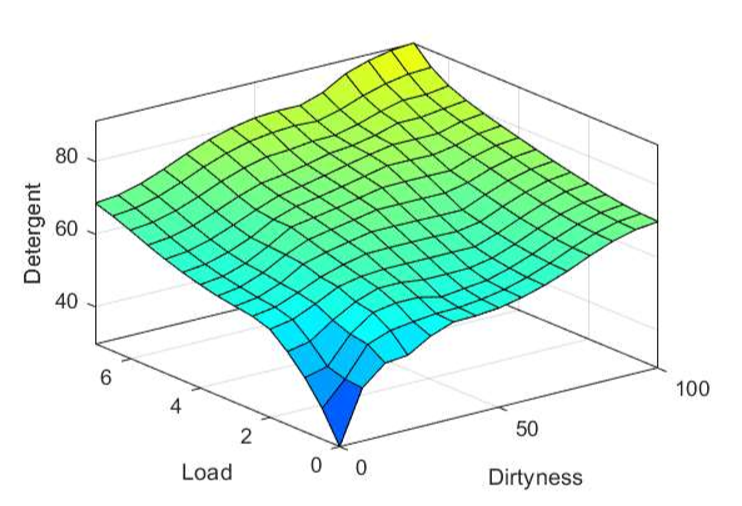
\includegraphics[width=.9\linewidth]{res/modelD_flat}
    \caption{ModelD - Increased Overlap}
    \label{fig:sub1}
  \end{subfigure}%
  \begin{subfigure}{.5\textwidth}
    \centering
    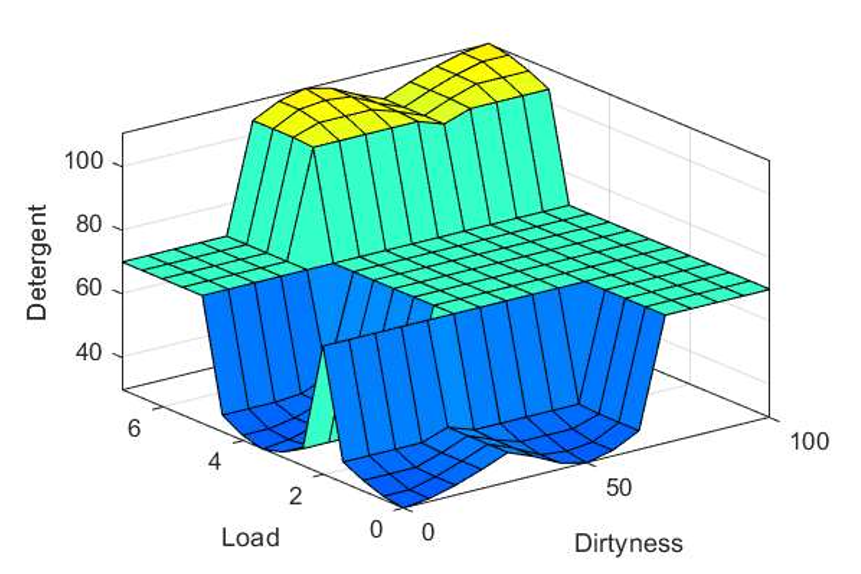
\includegraphics[width=.9\linewidth]{res/modelD_complex}
    \caption{ModelD - Decreased Overlap}
    \label{fig:sub2}
  \end{subfigure}
  \end{figure}

  % Change the settings according to the following parameters one at a time. How does this influence the behaviour of the system? Explain the meaning of the setting and describe your observations briefly. After each change, go back to the default settings.
  \item five

  % Change the input membership functions to be Gaussian rather than triangular for both inputs of Model CT. How does this influence the behaviour of the system? Explain briefly.
  \item six

\end{enumerate}


%%%%%%%%%%%%%%%%
%% Question 2 %%
%%%%%%%%%%%%%%%%

\section*{Question 2}

\begin{enumerate}[label=(\alph*)]

  % Show the input and output membership functions and the surfaces of your final (most preferred) system for the following 2 inputs - 1 output combinations: [Dirtiness, DirtType, CycleTime], [Load, Dirtiness, CycleTime] and [Load, DirtType, Detergent].
  \item one

  % How did you design the membership functions for the input variables? Why? (Consider the number of fuzzy sets, type of fuzzy sets, the support and the core of the fuzzy sets)
  \item two

  % What are the rules you created? Describe your reasoning.
  \item three

  % What are the settings for this system? Why do you prefer these settings? (Consider inference type, T/S-norm, aggregation, implication and defuzzification)
  \item four

  % By analyzing the surfaces in 2(a), discuss whether you have designed a washing machine that can solve the customers’ complaints.
  \item five

  % How can you further improve your design and why?
  \item six

\end{enumerate}


%%%%%%%%%%%%%%%%%%%%
%% Einde document %%
%%%%%%%%%%%%%%%%%%%%

\end{document}
